\documentclass[pdftex, a4paper, 12pt]{article}
\usepackage[ngerman]{babel}
\usepackage[utf8]{inputenc}
\usepackage[T1]{fontenc}
\usepackage{listings}
\usepackage{graphicx}
\usepackage{float}
\usepackage{here}
\usepackage{url}
\usepackage{capt-of}
\usepackage{multirow}
\usepackage{amsmath}
\usepackage{amssymb}
\usepackage{color}
\usepackage{titlesec}
\usepackage{hyperref}
\usepackage[scaled]{helvet}
\usepackage{fancyhdr}
\usepackage[usenames,dvipsnames]{xcolor}
\usepackage{geometry}
\usepackage{lscape}
%% acronyme
\usepackage{acronym}

%% Zeilenabstand einstellen:
\usepackage{setspace}


%%last packages DONT MODIFY - ask first


\geometry{a4paper,left=20mm,right=20mm, top=20mm, bottom=30mm}

%%fix für paragraph einrückung
\setlength{\parindent}{0in}

\renewcommand{\baselinestretch}{1.5}\normalsize

%spacing 
\onehalfspacing

\fancyhf{}
%Header
\fancyhead[R]{SEDA-WI-Proj-B}
\fancyhead[L]{Pflichtenheft}
%
%bottom
\fancyfoot[L]{SF GmbH}
\fancyfoot[C]{UnivIS 2.0}
\fancyfoot[R]{Seite: \thepage}

\renewcommand{\footrulewidth}{0.4pt}
\pagestyle{fancy}
\usepackage{hyperref}
\hypersetup{
    colorlinks ,
    citecolor=black,
    filecolor=black,
    linkcolor=black,
    urlcolor=black
}

%    \hypersetup{
%      colorlinks=false,
%      pdfborder={0 0 0}
%   }

\begin{document}
\bibliographystyle{alpha}

\begin{titlepage}

{\sffamily
\vspace*{2cm}
\begin{center}
	\bfseries
	\LARGE {Pflichtenheft der SF GmbH\\SEDA-WI-Proj-B}
\end{center}
\vspace{1cm}
\begin{center}

	% FILL IN YOUR DATA HERE
	{\Large\bfseries SF GmbH\\[5mm]}

	\begin{tabular}{ll}
		% AND HERE
		Denis Hamann & Matr.-Nr. 1684873 \\[3mm]

		Anna Kupfer & Matr.-Nr.  1491515\\[3mm]

		Hannes Stadler & Matr.-Nr. 1692114 \\[3mm]

		Christian Hindelang & Matr.-Nr. 1685285 \\[3mm]
		
		Mario Serno & Matr.-Nr. 1687104 \\[3mm]


	\end{tabular}\\[0.5cm]
	
{\scriptsize Otto-Friedrich-Universität Bamberg} \\[21pt]

%%\includegraphics[width=55pt]{images/uni-logo.jpg} \\[20pt]

{\footnotesize Version: v1.1 - \today }



\end{center}
}
\end{titlepage}


\newpage

\textcolor{MidnightBlue}{\tableofcontents}
%\tableofcontents

\textcolor{MidnightBlue}{\listoffigures}

\newpage
%Sections in separate files
\section{Einleitung}
\label{sec:Einleitung}

Die Vorliegende Arbeit enthält die Gesamtheit an notwendigen Spezifikationen die uns von der Otto-Friedrich-Universität übermittelt wurden. 
In diesen Vorgaben, dem Lastenheft, wurden Ergebnisse aus eigens angeführten Ermittlungen zu den individuellen Anforderungen durch Fragebögen, Selbstaufschreibungen sowie Feldbeoachtungen [Balz09, S.303] zur aktuellen und gewünschten Einsatzsituation der neuen Software UniVis 2.0 zusammengestellt.
Nach der ausführlichen Sichtung aller Unterlagen und einer ersten Vorstudie der Anforderungen konnte dieses Pflichtenheft erstellt werden. In diesem finden Sie jegliche fachliche Definitionen und Anforderungen, die im Zusammenhang mit der gewünschten Software UniVis 2.0 und den gewünschten Funktionen und Leistungen stehen.
\\
\\
Aus diesem Grund werden zunächst die unterschiedlichen Zielbestimmungen, der präzise Produkteinsatz sowie die gesamte Umgebung (Soft-, Hard-, Orgware und Produkt-Schnittstellen) erläutert.
Dem folgen detaillierte Spezifikationen zu den Funktionen, Daten und Leistungen. Um erste Eindrücke zu sammeln und somit zu vermitteln werden Anforderungen an die Benutzeroberfläche sowie erste Prototyp-User-Interfaces vorgestellt. Das Pflichtenheft schließt mit qualitätsbezogenen Zielbestimmungen, globalen Testszeanrien und genauen Angaben zur Entwicklungsumgebung.
Weiter Ergänzungen sowie ein Glossar dienen der Komplettierung und Vermittlung einer besseren Verständlichkeit des vorliegende Dokuments.


\subsection{Definitionen}
\label{sec:Definitionen}

In diesem Abschnitt werden Abkürzungen und Begrifflichkeiten erläutert, die im Pflichtenheft verwendet werden. \\[0.25cm]

\begin{tabular}{p{1.5cm}p{14.5cm}}

	/X0/	& Eine derartige Kennzeichnung wird im Pflichtenheft für die Kennzeichnung von Software-Merkmalen verwendet. Anstelle des "X" steht die Abkürzung des Merkmals. "Z" kennzeichnet Zielbestimmungen, "F" Funktionen, "D" Daten, "L" Leistungen, "B" die Benutzeroberfläche, "Q" qualitative Bestimmungen und "T" Testszenarien. Anstelle der "0" steht die Nummer des jeweiligen Merkmals.  \\
	/XW0/	& Diese Kennzeichnung entspricht der wie sie bei "/X0/" beschrieben ist, das zusätzliche "W" signalisiert allerdings, dass es sich um ein wünschenswertes Merkmal handelt, dass je nach Entwicklungsaufwand und Dringlichkeit ggf. nicht in der ersten Version der Software implementiert sein wird. \\

\end{tabular}
\newpage
\section{Preamble}
\label{sec:preamp}

We'd like to address the reader of this documentation before going into the details of this documentation that the project itself encountered several challenges which couldn't all be solved in a satisfying way. These lead to a program with a limited functionality and a documentation with some major gaps. For reasons and the progress itself which lead to this situation please refer to chapter 8.
\newpage
\section{Produkteinsatz}
\label{sec:Produkteinsatz}

\subsection*{(Mario Serno)}

Das Produkt dient der Verwaltung von Räumen, Lehrveranstaltungen und Systemnutzer am Standort Erba der Otto-Friedrich-Universität Bamberg. Insbesondere soll der Raumbedarf der Lehrstühle und die Raumplanung durch die Hausverwaltung effektiv koordiniert werden. Des Weiteren soll den Studenten eine Möglichkeit geboten werden, sich einen Stundenplan zu erstellen.

\subsection{Anwendungsbereiche}
\begin{tabular}{p{1.5cm}p{14.5cm}}	
	 /P10/& Das Produkt wird intern an der Otto-Friedrich-Universität Bamberg eingesetzt. \\[0.25cm]
\end{tabular}


\subsection{Zielgruppen}
\begin{tabular}{p{1.5cm}p{14.5cm}}	
	 /P20/& Zielgruppen des Produktes sind Lehrstühle, deren Mitarbeiter, die Hausverwaltungsmitarbeiter und Studenten der der Otto-Friedrich-Universität Bamberg am Standort Erba. \\[0.25cm]
\end{tabular}


\subsection{Betriebsbedingungen}
\begin{tabular}{p{1.5cm}p{14.5cm}}	
	 /P30/& Das Produkt wird auf den Clients der Hausverwaltung, Lehrstühle und PC-Pools ausgeführt. \\[0.25cm]
\end{tabular}

\begin{tabular}{p{1.5cm}p{14.5cm}}	
	 /P40/& Das System ist so zu konzipieren, dass die einzelnen Anwendungsinstanzen über eine gemeinsame Datenbasis (PostgreSQL-Server) kommunizieren können. \\[0.25cm]
\end{tabular}

\begin{tabular}{p{1.5cm}p{14.5cm}}	
	 /P50/& Die tägliche Betriebszeit des Produktes erstreckt sich Montag bis Freitags jeweils von 08:00 bis 20:00 Uhr. Eine Nutzung am Wochenende ist nicht vorgesehen. \\[0.25cm]
\end{tabular}

\begin{tabular}{p{1.5cm}p{14.5cm}}	
	 /P60/& Zu Beginn jedes Semesters wird die Lauffähigkeit des Produktes durch einen Administrator über einen Zeitraum von drei Wochen beobachtet. Nach Ablauf dieses Zeitraums ist ein unbeaufsichtigter Betrieb vorgesehen. \\[0.25cm]
\end{tabular}

\newpage
\section{Produktumgebung}
\label{sec:Produktumgebung}

\subsection*{(Denis Hamann)}

Im Folgenden wird die Umgebung beschrieben, in der die finale Software eingesetzt werden soll.
Die Produktumgebung umfasst die Basismaschinen und die Systemumgebung, getrennt nach Software, Hardware und
Produktschnittstellen. Zusätzlich werden im Bereich Orgware die zugehörigen organisatorischen Randbedingungen beschrieben.

\subsection{Software}
\label{subsec:software}

Die Software beschreibt die vorzuhaltende Software-Umgebung um eine problemlose Ausführung des Programms sicherzustellen.\\

\begin{tabular}{p{1.5cm}p{14.5cm}}

	 /PU10/	&  Als Betriebssystem kommt Windows 7 (Professional, x64 - 64bit) zum Einsatz. Dieses hat die neusten Updates vorzuweisen und eine gängige sowie aktuelle Antiviren Lösung installiert zu haben.\\[0.25cm]

\end{tabular}

\begin{tabular}{p{1.5cm}p{14.5cm}}

	 /PU20/	&  Im Bereich der Laufzeitumgebung wird auf die Java Virtual Machine Version 7 von Oracle gesetzt.
Hierzu ist das entsprechende Java Runtime Environment (JRE) in Version 7 vorzuhalten. Es muss sichergestellt werden, dass die entsprechenden Klassenpfade, sowie Systempfade gesetzt sind, sodass der Prozess java als auch javaw im CLI bekannt ist. Darüber hinaus müssen .jar-Dateien mit der JRE verknüpft sein um einen Start der Anwendung per Doppelklick zu gewährleisten. Entsprechende Einstellungen sind notfalls in der Registry vorzunehmen [vgl. Kapitel \ref{subsec:jarreg}].\\[0.25cm]

\end{tabular}

\begin{tabular}{p{1.5cm}p{14.5cm}}

	 /PU30/	&  Die Datenbank welche in Verbindung mit der Software eingesetzt wird, stellt PostgreSQL in Version 9.2.1 dar.
Es muss sichergestellt werden, dass die betreffenden PCs welche die neue UnivIS Software verwenden sollen für die Datenbank freigeschaltet sind (Freigabe der jeweiligen IPs).\\[0.25cm]

\end{tabular}


\begin{tabular}{p{1.5cm}p{14.5cm}}

	 /PU40/	&  Zusätzlich soll sichergestellt werden, dass entsprechende Netzwerk-Einstellungen (Firewalls, Router) eine ordnungsgemäße Verbindung zwischen Anwendungs-PC und Datenbank erlauben.\\[0.25cm]

\end{tabular}


\begin{tabular}{p{1.5cm}p{14.5cm}}

	 /PU50/	&  Das Programm wird auf die Swing-Komponenten von Java setzten, daher ist es notwendig sicher zustellen, dass eine entsprechende Shell vorhanden ist.
Als Oberfläche wird auf die Standard Fensteroberfläche von Windows 7 (shell: explorer.exe) gesetzt. Kiosk-Systeme sind als Benutzeroberfläche nicht vorgesehen.\\[0.25cm]

\end{tabular}


\subsection{Hardware}
\label{subsec:hardware}


\begin{tabular}{p{1.5cm}p{14.5cm}}

	 /PU60/	&  Die Software soll auf IBM-Kompatiblen Computern der Intel x86 Architektur ausgeführt werden.
Um sicher zu gehen, dass die Anwendung ausreichend schnell ausgeführt wird, werden nachfolgende Systemvoraussetzungen empfohlen:\\

	&CPU: 1Ghz\\
	&RAM: 1GB\\
	&HDD: 100MB\\
	&Peripherie: Maus \& Tastatur\\
	&\\
	&Zusätzlich muss sichergestellt werden, dass ein entsprechender Netzwerkanschluss für die Verbindung zum Datenbankserver vorhanden ist.\\[0.25cm]


\end{tabular}

\begin{tabular}{p{1.5cm}p{14.5cm}}

	 /PU70/	&  Entsprechende Netzwerkhardware (Router, Switch, Patchpannel, Firewall, Netzwerkkabel) zur Verbindung der Computer mit dem Datenbankserver werden vorausgesetzt.\\[0.25cm]


\end{tabular}



\subsection{Orgware}
\label{subsec:orgware}

\begin{tabular}{p{1.5cm}p{14.5cm}}

	 /PU80/	&  Für die Entwicklung der Software wird vorausgesetzt, dass jeweils ein involvierter Mitarbeiter der unterschiedlichen Organisationsbereiche der Universität zur Beantwortung von fachspezifischen Fragen zur Verfügung steht. Darüber hinaus ist für Arbeiten vor Ort ein entsprechender Platz zu stellen.\\[0.25cm]


\end{tabular}

\begin{tabular}{p{1.5cm}p{14.5cm}}

	 /PU90/	&  Benutzerhandbücher werden, sofern benötigt, in elektronischer Form (PDF) ausgeliefert. Sie beschreiben die grundlegenden Funktionen der Software.\\[0.25cm]


\end{tabular}

\begin{tabular}{p{1.5cm}p{14.5cm}}

	 /PU100/	&  Der Auftraggeber stellt sicher, dass dem Auftragsnehmer entsprechende Informationen zur Verfügung gestellt werden, um eine ordnungsgemäße Autorisierung und Authentifizierung der Benutzer sicherzustellen.\\[0.25cm]


\end{tabular}

\begin{tabular}{p{1.5cm}p{14.5cm}}

	 /PU110/	&  Die Datenbank (PostgreSQL) muss auf einem entsprechenden Server installiert sein und als Dienst laufen. Es muss sicher gestellt werden, dass entsprechende Router und Firewalls konfiguriert sind und eine Verbindung in beide Richtungen möglich ist, um eine Persistierung der Daten zu ermöglichen. Die Bereitstellung, sowie entsprechende Verfügbarkeit stellt der Auftraggeber sicher\\[0.25cm]


\end{tabular}

\begin{tabular}{p{1.5cm}p{14.5cm}}

	 /PU120/	&  Es wird davon ausgegangen, dass die Hausverwaltung, sowie die Dozenten entsprechende Informationen zu Räumen und Lehrveranstaltungen korrekt und zeitnah in das System einpflegen um eine sinnvolle Nutzung zu ermöglichen.\\[0.25cm]


\end{tabular}




\subsection{Produkt-Schnittstellen}
\label{subsec:productinterface}

\begin{tabular}{p{1.5cm}p{14.5cm}}

	 /PU130/	&  Das Produkt beinhaltet lediglich eine Schnittstelle zur Datenbank wie in Kapitel \ref{subsec:software} beschrieben. Über diese findet die Persistierung der Daten, sowie die Abfrage komplexer Anfragen statt.
Schnittstellen mit der zukünftig geplanten Weboberfläche, sowie Mobilen Anwendung erfolgt nicht über die Software direkt sondern über die gemeinsame Datenbank. Die dort vorliegende Datenstruktur ist allen weiteren Anwendungen bekannt und ermöglicht so eine reibungslose Interaktion zwischen den Systemen.
Parallele Sitzungen der Software werden ebenfalls über die Datenbank synchron gehalten. D.h. trägt Benutzer1 an Workstation1 eine neue Lehrveranstaltung ein, so ist diese auch in Workstation2 bei Benutzer2 bei entsprechender Einstellung zu sehen. Eine direkte Kommunikation zwischen den einzelnen Instanzen der Software findet nicht statt.\\[0.25cm]


\end{tabular}



\subsection{Zukünftige Entwicklungen}
\label{subsec:zukunftentw}

\begin{tabular}{p{1.5cm}p{14.5cm}}

	 /PU140/	&  Wie bereits im Lastenheft angemerkt ist vorgesehen die Software später über den Standort hinaus zu verwenden.
Neben der Ausweitung der Standorte sollen die Zugriffsmöglichkeiten auf das System um ein Webinterface, sowie eine Mobile Anwendung erweitert werden.
Diese Entwicklungen werden in der erstellten Software berücksichtigt und entsprechend umgesetzt.\\[0.25cm]


\end{tabular}

\begin{tabular}{p{1.5cm}p{14.5cm}}

	 /PU150/	&  Um sicherzustellen, dass die spätere Erweiterung problemlos möglich ist, erhält der Auftraggeber entsprechend eine Dokumentation des Quellcodes, sowie der Datenbank bzw. dessen konkrete Relationen.
Für das Ziel das bestehende UnivIS zu einem späteren Zeitpunkt zu ersetzten sollte dementsprechend ein Change-Management Ansatz gefahren werden, in diesem unter anderem auch die Schulung der späteren Benutzer erfolgen sollte. \\[0.25cm]


\end{tabular}


%Das System soll zunächst ausschließlich am Standort ERBA zum Einsatz
%kommen. Sollte es einer Evaluierung nach einem Zeitraum von vier Semestern
%standhalten, plant die Universität den Einsatz auf weitere Standorte
%auszudehnen sowie den Einsatz im Web und auf mobilen Endgeräten. Fernziel
%ist die Ablösung des bestehenden Systems .
\newpage
\section{Preamble}
\label{sec:preamp}

We'd like to address the reader of this documentation before going into the details of this documentation that the project itself encountered several challenges which couldn't all be solved in a satisfying way. These lead to a program with a limited functionality and a documentation with some major gaps. For reasons and the progress itself which lead to this situation please refer to chapter 8.
\newpage
%-------------------------------
\section{Produktdaten}
\label{sec:Produktdaten}
%-------------------------------

\begin{quote}
\begin{tabular}{p{1.5cm}p{14.5cm}}


	 /D10/	& \textbf{Datentyp:} Räume \\
				& \textbf{Attribute:} Raum ID \textsl{(systemintern)}, Raumnummer, Gebäude, Stockwerk, Sitzplätze, PC-Plätze, Beamer, Visualizer, Overheads, Tafeln, Whiteboards  \\[0.25cm]

\end{tabular}


\begin{tabular}{p{1.5cm}p{14.5cm}}
		
	 /D20/	& \textbf{Datentyp:} Lehrstühle \\
				& \textbf{Attribute:} Lehrstuhl ID \textsl{(systemintern)}, Lehrstuhlname, Lehrstuhlinhaber, Fakultät, (Haupt-)Gebäude, (Haupt-)Stockwerk  \\[0.25cm]

\end{tabular}


\begin{tabular}{p{1.5cm}p{14.5cm}}
					
	 /D30/	& \textbf{Datentyp:} Benutzer \\
				& \textbf{Attribute:} Benutzer ID \textsl{(systemintern)}, Benutzerkennung, Passwort (Hash), Salt, E-Mail, Benutzerzugehörigkeit (Verwaltung, betreffender Lehrstuhl, wünschenswerterweise auch Student), Vorname, Nachname, letzter Login  \\[0.25cm]

\end{tabular}


\begin{tabular}{p{1.5cm}p{14.5cm}}
	
	 /D50/	& \textbf{Datentyp:} Lehrveranstaltungen \\
				& \textbf{Attribute:} Veranstaltungs ID \textsl{(systemintern)}, Benutzer ID (Dozent), Veranstaltungskurzbezeichnung, Veranstaltungsname, Semester, Benötigte SWS, Art (Vorlesung|Übung|Tutorium), Freigabe durch Dozent, Beschreibung (Tag, Zeiteinheiten, etc. wird über "Raumbelegung (/D60/)" ermittelt, wo für jede Zeiteinheit ein Eintrag erstellt wird und Veranstaltungen mehrere Einträge pro Semester buchen können.) \\[0.25cm]

\end{tabular}


\begin{tabular}{p{1.5cm}p{14.5cm}}
					
	 /D60/	& \textbf{Datentyp:} Raumbelegungen (aller Freigabestatus-Arten) \\
				& \textbf{Attribute:} Belegungs ID \textsl{(systemintern)}, Veranstaltungs ID (Lehrveranstaltung), Raum ID, Semester, Tag, Zeiteinheit, Freigabestatus (unbearbeite|freigegeben|abgelehtn|gegenvorschlag), Freigabenachricht (Falls ein Vorschlag abgelehnt wurde und dies nun ein reservierter Vorschlag des Status "gegenvorschlag" ist), Kommentar  \\[0.25cm]

\end{tabular}


\begin{tabular}{p{1.5cm}p{14.5cm}}
		
	 /DW70/& \textbf{Datentyp:} Studentenbelegungen \\
				& \textbf{Attribute:} Studenten-Belegungs ID \textsl{(systemintern)}, Benutzer ID (Student), Belegungs ID (freigegebene Lehrveranstaltung) \\[0.25cm]

\end{tabular}


\begin{tabular}{p{1.5cm}p{14.5cm}}
					
	 /DW80/& \textbf{Datentyp:} Ticker-Nachricht \\
				& \textbf{Attribute:} Meldungs ID \textsl{(systemintern)}, Meldungstext, Start-Datum, End-Datum, exklusiv für Lehrstuhl ID ('null' wenn für alle), exklusiv für Veranstaltungs ID ('null' wenn für alle), exklusiv für Raum ID ('null' wenn für alle) \\[0.25cm]
		
\end{tabular}


In Structured-Entity-Relationship-Modell (SERM) wird der Zusammenhang der oben spezifizierten persistent zu speichernden Daten verdeutlicht. \\

\begin{figure}
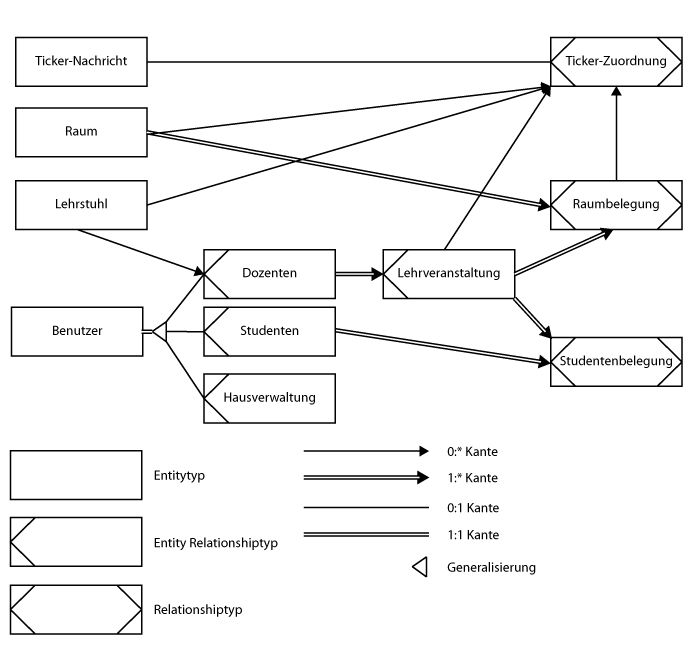
\includegraphics[width=13cm, height=14cm]{./images/section_5/dbserm}
\caption{SERM der Daten-Architektur}
\label{fig:dbserm}
\end{figure}

Wie zu sehen ist, existieren sowohl Räume als auch Lehrstühle als eigenständige Einheiten (Entity). Benutzer können einem Lehrstuhl zugeordnet werden, womit sie der Klasse "Dozent" entsprechen. Sie können aber auch der Klasse "Verwaltung" oder "Student" angehören und somit keinem Lehrstuhl zugeordnet werden. Lehrveranstaltungen müssen einem Benutzer zugeordnet werden, der (allein an der Grafik nicht erkennbar) ein der Klasse "Dozent" angehören muss. Eine Raumbelegung ist keine Einheit sondern eine Zuordnung (Relationship) und muss einer Lehrveranstaltung und einem Raum zugeordnet werden können. Die Zuordnung Studentenbelegung muss einem Benutzer (der Klasse "Student") und einer Raumbelegung zugeordnet werden können. Ticker-Nachrichten können einem Raum, einer Lehrveranstaltung oder einem Lehrstuhl zugeordnet werden, nichts davon ist aber zwingend. \\


\end{quote}
\newpage
%-------------------------------
\section{Produktleistung}
\label{sec:Produktleistung}
%-------------------------------


\begin{tabular}{p{1.5cm}p{14.5cm}}


	 /L10/	& Alle Daten, die im vorherigen Abschnitt aufgelistet sind, müssen, sofern sie realisiert werden, persistent mittels einer SQL-Datenbank (erreichbar und verwaltet durch einen PostgreSQL-Server) gespeichert werden. \\[0.25cm]
	 
\end{tabular}


\begin{tabular}{p{1.5cm}p{14.5cm}}
						
	 /L20/	& Bei allen Prozess mit Dateneingabe-Funktionen erhalten Nutzer aussagekräftige Fehlermeldungen, sollte ihr Prozess nicht ordnungsgemäß durchgeführt werden können. \\[0.25cm]
	 
\end{tabular}


\begin{tabular}{p{1.5cm}p{14.5cm}}
						
	 /L30/	& Die Realisierung erfolgt als Java-Anwendung, so dass ein möglicher Betrieb auf allen gängigen PCs der Universität sichergestellt ist. \\[0.25cm]

\end{tabular}


\begin{tabular}{p{1.5cm}p{14.5cm}}
						
	 /L40/	& Die Programmarchitektur richtet sich nach dem MVC-Modell, wobei eine saubere untergliederung zwischen den Schichten gewährleistet wird, sowie ein hohes Maß an Modularität erreicht wird. Dieses erlaubt es auch verhältnismäßig einfach Erweiterungen zu einem späteren Zeitpunkt zu erstellen. \\
	 &	Die erste Version der Anwendung soll aus folgenden Modulen bestehen: \\
	 &	\textbf{CoreGUI:} Hier wird die Start-Routine sowie der Startbildschirm der Anwendung realisiert. Die Funktion /F01/ und /F60/ werden von diesem Modul umgesetzt.\\
	 &	\textbf{Verwaltung:} Hier wird die Anzeige für Verwaltungsmitglieder umgesetzt, die die Funktion /F10/, wünschenswerterweise /FW21/, /F40/, /F50/, /F51/, /F80/ und /F90/ realisiert.\\
	 &	\textbf{Dozenten:} Hier wird die Anzeige für Dozenten umgesetzt, die die Funktion /F20/, wünschenswerterweise /FW21/, /F30/, /F140/, /F150/ und /F70/ realisiert.\\
	 &	\textbf{Stundenplan:} Hier wird die Anzeige für den Stundenplan von Studenten umgesetzt, die die Funktion /F130/ realisiert.\\
	 &	\textbf{Raumplan:} Hier wird die Anzeige für Mitglieder der Verwaltung (und ggf. andere) von Räumen und deren Belegung umgesetzt, die die Funktion /F120/ realisiert.\\
	 &	\textbf{Studentenprofil (wünschenswert):} Hier wird die Anzeige für Studenten umgesetzt, die die Funktion /FW61/ realisiert.\\[0.25cm]

\end{tabular}


\begin{tabular}{p{1.5cm}p{14.5cm}}
					
	 /L50/	& Es wird eine Nutzerauthentifizierung realisiert, die es gewährleistet, dass nur berechtigte Nutzer Änderungen durchführen. Um Missbrauch ausschließen zu können, sollte allerdings eine Middleware (die großteils die Model- und Controller-Schicht abdeckt) zwischen Datenbank und Client (der haupsächlich die View-Schicht umsetzt) realisiert werden. In diesem Fall sollte die Kommunikation zwischen Client und Middleware durch SSL (mithilfe von javax.net.ssl.* und javax.rmi.ssl.*) abgesichert werden. \\[0.25cm]
	
\end{tabular}


\begin{tabular}{p{1.5cm}p{14.5cm}}
					
	 /L60/	& Zeitliche Spezifikationen (Abgleich mit Christian) \\[0.25cm]
	
\end{tabular}



%################################
% \end{document}
%################################
\newpage
\section{Benutzeroberfläche}
\label{sec:Benutzeroberfläche}

\subsection*{(Anna Kupfer)}

Dieser Abschnitt beschäftigt sich mit der grundlegenden Gestaltung der Benutzeroberfläche für die unterschiedlichen Nutzer [vgl. \cite{UniRos12b}, \cite{UniRos12c}, \cite{balz1996} \cite{Balzert2009}, \cite{Schae12}, \cite{Jurij07}]. Zunächst werden allgemeine Anforderungen definiert worauf spezifische zum Bildschirm- und Drucklayout sowie der Tastaturbelegung folgen. Das Kapitel schließt mit einer ausführlichen Betrachtung der Dialogstruktur und untermalt diesen Punkt mit Screenshots zum ersten GUI-Prototypen.


\begin{tabular}{p{1.5cm}p{14.5cm}}
 /B10/	& Fensterlayout, Dialogstruktur und Mausbedienung entsprechen dem Windows-Gestaltungs-Regelwerk [vgl. \cite{microsoft1995windows}]. \\[0.25cm]	 
\end{tabular}

\begin{tabular}{p{1.5cm}p{14.5cm}}
 /B11/	& Sämtliche Daten sind passwortgeschützt und dürfen nur von autorisierten Mitarbeitern des Lehrstuhls bearbeitet werden. \\[0.25cm]	 
\end{tabular}


\subsection{Bildschirmlayout}

\begin{tabular}{p{1.5cm}p{14.5cm}}
 /B20/	& Eine übersichtliche Gestaltung der Funktionen und intuitive Nutzung durch ein angepasstes Bildschirmlayout soll vorherrschen. \\[0.25cm]	 
\end{tabular}	

\begin{tabular}{p{1.5cm}p{14.5cm}}
 /B30/	& Standardmäßig startet das Programm mit einer Suchmaske. Weitere Funktionen sind via Tabs und einem Login erreichbar. \\[0.25cm]	 
\end{tabular}

\begin{tabular}{p{1.5cm}p{14.5cm}}
 /BF40/	& Individuelle Anpassungsfähigkeit des Bildschirmlayouts an die Fenstergröße sollte möglich sein. \\[0.25cm]	 
\end{tabular}

\subsection{Drucklayout}

\begin{tabular}{p{1.5cm}p{14.5cm}}
 /B50/	& Nicht angemeldete Nutzer können über die Auswahl verschiedener Lehrveranstaltungen einen Stundenplan im PDF-Format in Din-A4 Größe erzeugen lassen [siehe Abbildung \ref{img:stundenplanAlle}]. \\[0.25cm]	 
\end{tabular}

\begin{tabular}{p{1.5cm}p{14.5cm}}
 /B60/	& Die Hausverwaltungsnutzer können Raumpläne im PFD-Format in Din-A4 Größe erzeugen lassen (ähnlich der Studenten-, Dozenten-, und Lehrstuhlstundenpläne). \\[0.25cm]	 
\end{tabular}

\begin{tabular}{p{1.5cm}p{14.5cm}}
 /B70/	& Mitarbeiter der Lehrstühle können personen- oder lehrstuhlbezogene Wochenpläne in einem PDF-Format in Din-A4 Größe exportieren[siehe Abbildungen \ref{img:StundenplanDoz}, \ref{img:LehrstuhlplanDoz}]. \\[0.25cm]	 
\end{tabular}

Hier einige Beispiele zur Ausgabe des Stundenplans für Studenten, Dozenten und Lehrstühle:
\begin{figure}[H]
\begin{center}
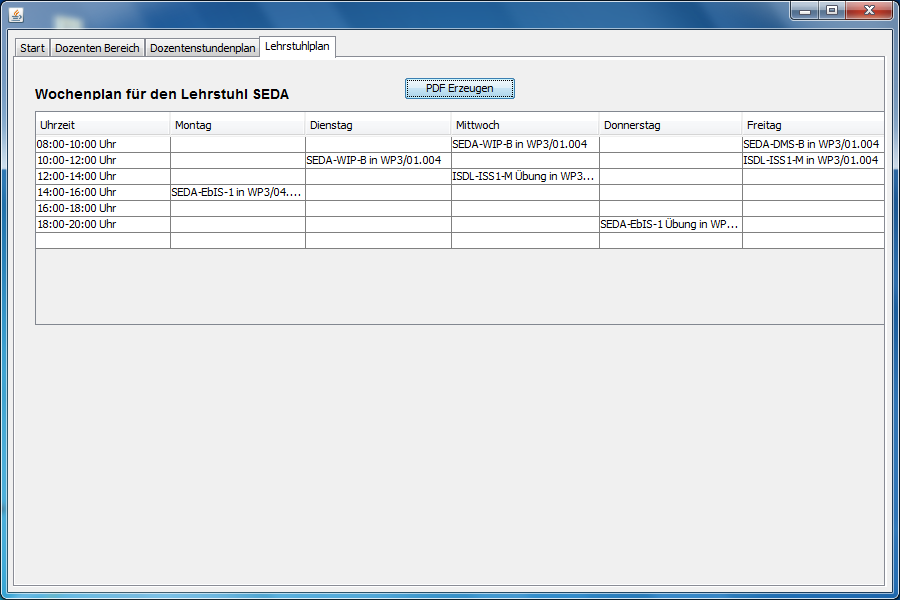
\includegraphics[width=150mm]{images/section_7/DozentenLehrstuhlplan.PNG}
\caption{Lehrstuhlplan}
\label{img:LehrstuhlplanDoz}
\end{center}
\end{figure}

\begin{figure}[H]
\begin{center}
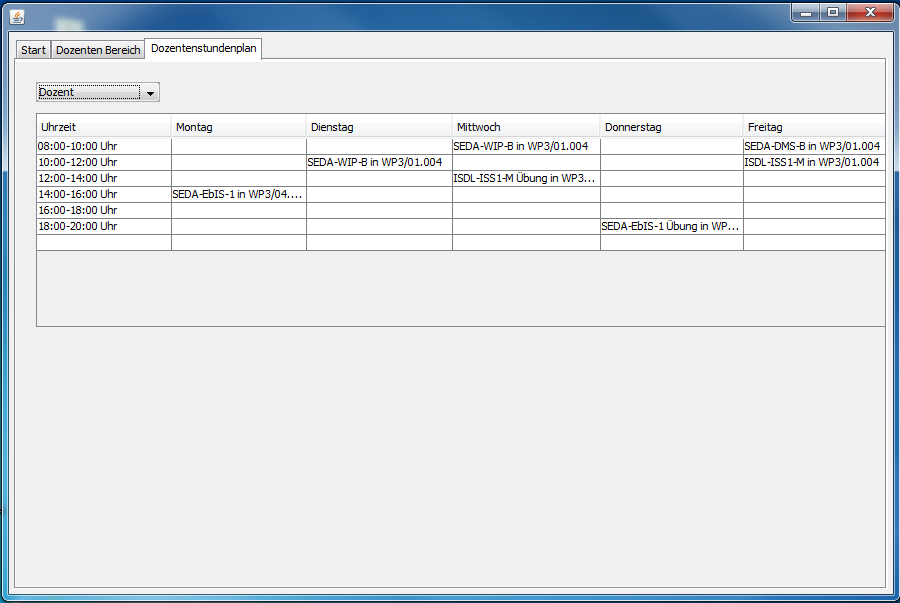
\includegraphics[width=150mm]{images/section_7/DozentenStundenplan.PNG}
\caption{Dozentenstundenplan}
\label{img:StundenplanDoz}
\end{center}
\end{figure}

\begin{figure}[H]
\begin{center}
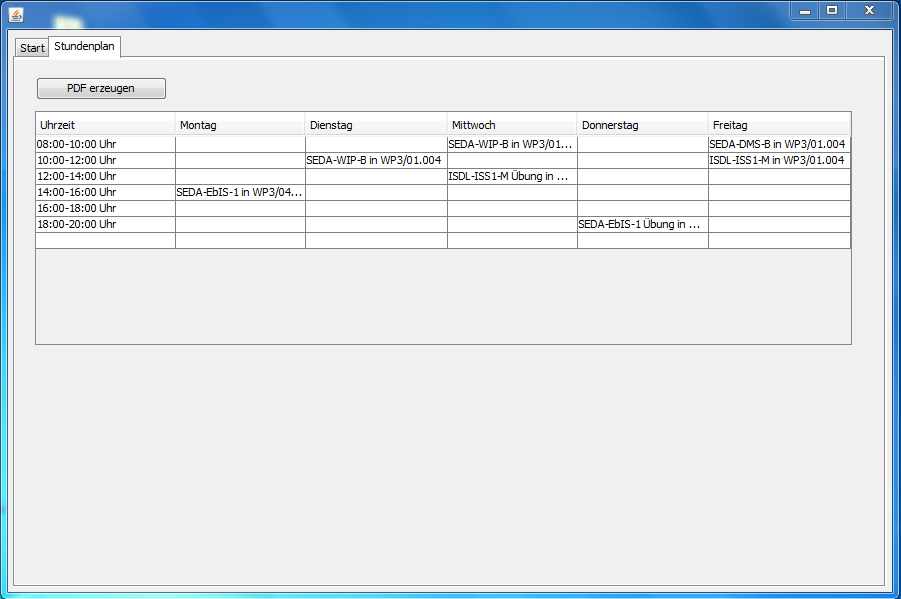
\includegraphics[width=150mm]{images/section_7/HauptseiteAlleStundenplan.PNG}
\caption{Stundenplananzeige, rollenunabhängig}
\label{img:stundenplanAlle}
\end{center}
\end{figure}
 
\subsection{Tastaturbelegung}

\begin{tabular}{p{1.5cm}p{14.5cm}}
 /B80/	& Die Benutzeroberfläche ist auf eine Bedienung mittels Tastatur und Maus auszulegen. Benutzer in der Studentenrolle können keine Eingaben mittels der Tastatur vornehmen. Dozenten und die Hausverwaltung benötigen die Tastatur um verschiedene Funktionen auszuführen. \\[0.25cm]	 
\end{tabular}

\begin{tabular}{p{1.5cm}p{14.5cm}}
 /BF81/	& Mögliche individuelle, nicht dem Windows Standard entsprechende, Tastaturbelegungen sind ein mögliches  Wunschkriterium. \\[0.25cm]	 
\end{tabular}


\subsection{Dialogstruktur}

\begin{tabular}{p{1.5cm}p{14.5cm}}
 /B90/	& Zu Beachten ist: ISO 9241-10: 1996 bzgl. der ergonomischen Anforderungen für Bürotätigkeiten mit Bildschirmgeräten, Teil 10: Grundsätze der Dialoggestaltung. \\[0.25cm]	 
\end{tabular}

\begin{tabular}{p{1.5cm}p{14.5cm}}
 /B91/	& Folgende Rollen sind zu unterscheiden: \\[0.25cm]	 
\end{tabular}\\


\begin{table}[H]
\begin{tabular}{l|l}
Rolle&Rechte\\
\hline
\hline
Student & (F01), F60 , FW61, F130 \\
\hline
Dozent & F01, F20, FW21, F30, F70, F140, F150  \\
\hline
Verwaltungsangestellter & F01, F10, FW21, F40, F50, F51, F80, F90,  \\
\hline
Alle & F01, F100, F110, F120
\end{tabular}
\end{table}
% line
%line

Nachfolgend wird die Dialogstruktur durch den GUI-Prototypen verdeutlicht, um die Benutzeroberfläche vorzustellen und zu erläutern.
Im Anschluss an den Programmstart erscheint die Startseite des UnivIS 2.0 [siehe Abbildung \ref{img:hauptseite}]. Hier können unangemeldete Nutzer (vor allem Stundenten) über Dropdown Menüs verschiedene Lehrveranstaltungen suchen und diese anschließend mittels dem "`+"'-Button die Lehrveranstaltungen zur Stundenplan-Sammlung hinzufügen  [siehe /F60/]. Schon bei der ersten Verwendung des "`+"'-Buttons öffnet sich ein neuer Tab, in welchem der Stundenplan gemäß der selektierten und gesammelten Lehrveranstaltungen ausgegeben wird. Anhand der Radiobuttons (Lehrveranstaltungen und Räume) können gleichzeitig Belegungen einzelner Räume selektiert und weiterhin im Stundenplan-Tab visualisiert werden [siehe /F100/, /F130/].
Im linken Bereich der Benutzeroberfläche befindet sich der Live-Ticker [siehe /F110/], über welchem anstehende Lehrveranstaltungen oder sonstige Informationen ausgegeben werden.
Im unteren linken Bereich befindet sich der Login [siehe /F01/] für Dozenten und die Hausverwaltung (evtl. auch einmal für Studenten) [siehe /FW61/] mittels Benutzerkennung/name und Passwort.
Im Falle einer erfolgreichen Anmeldung als Hausverwaltungsmitglied folgt die Startseite für Hausverwaltungsmitarbeiter [siehe Abbildung \ref{img:hauptseiteVerwaltung}]. 
Sie haben einen unmittelbaren Überblick über alle Raumanfragen und können diese sogleich bearbeiten (freigeben, ablehnen oder etwaige Konflikte lösen) [siehe /F80/, /F40/].
Im linken Bereich bleibt Platz für einen personalisierten Live-Ticker. Weiter unten können die Benutzer auf weitere Aktionen zugreifen.
Werden weitere Aktionen ausgeführt gelangt der Benutzer zu weiteren Listen und kann jeweils Lehrstühle, Nutzer und Räume verwalten (hinzufügen, bearbeiten oder löschen) [siehe /F10/, /F50/, /F51/, /F90/, /F100/ und siehe Abbildungen \ref{img:LehrstuhlVerw} und \ref{img:NutzerVerw}]. Bei der Raumverwaltung kann zusätzlich ein Raumplan erstellt werden [siehe /F120/ und siehe Abbildung \ref{img:RaumVerw}].
Eine letzte abdingbare Funktion wäre die Bearbeitung des LiveTickers um bspw. Dozenten verwaltungstechnische Nachrichten anzeigen lassen zu können [siehe /FW21/].
\begin{figure}[H]
\begin{center}
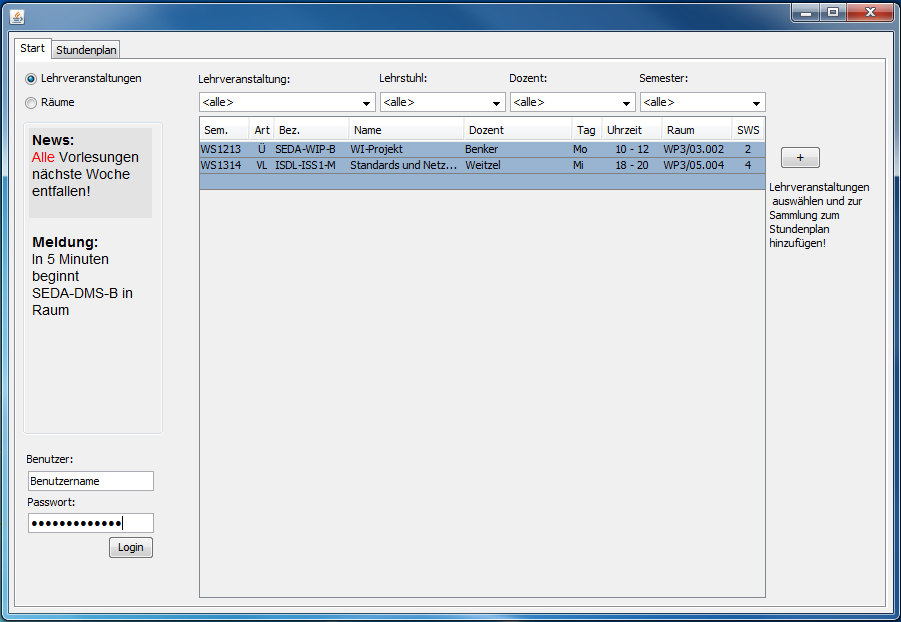
\includegraphics[width=150mm]{images/section_7/HauptseiteAlle.PNG}
\caption{GUI Startseite, rollenunabhängig}
\label{img:hauptseite}
\end{center}
\end{figure}


\begin{figure}[H]
\begin{center}
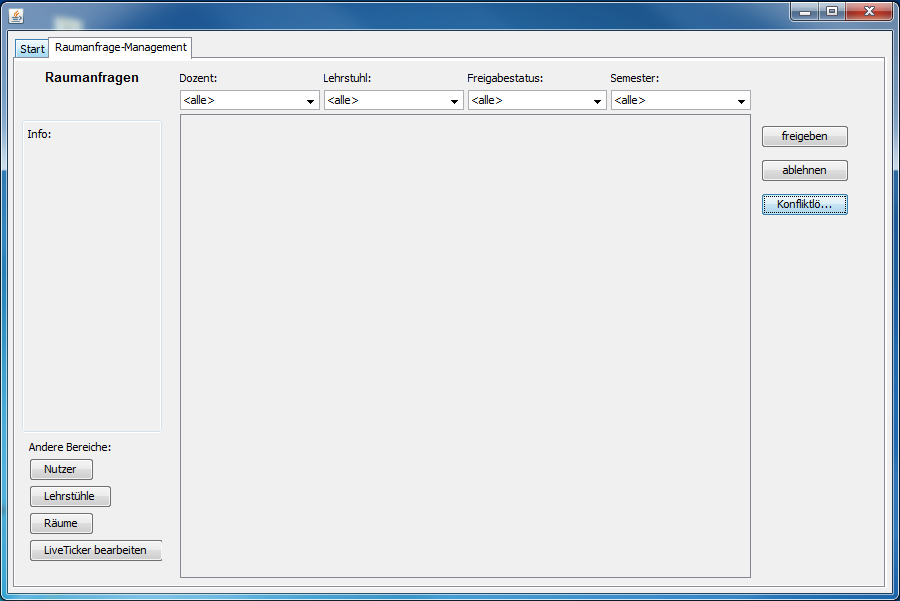
\includegraphics[width=150mm]{images/section_7/VerwaltungHauptseite.PNG}
\caption{Startseite für authentifizierte Benutzer der Hausverwaltung}
\label{img:hauptseiteVerwaltung}
\end{center}
\end{figure}

\begin{figure}[H]
\begin{center}
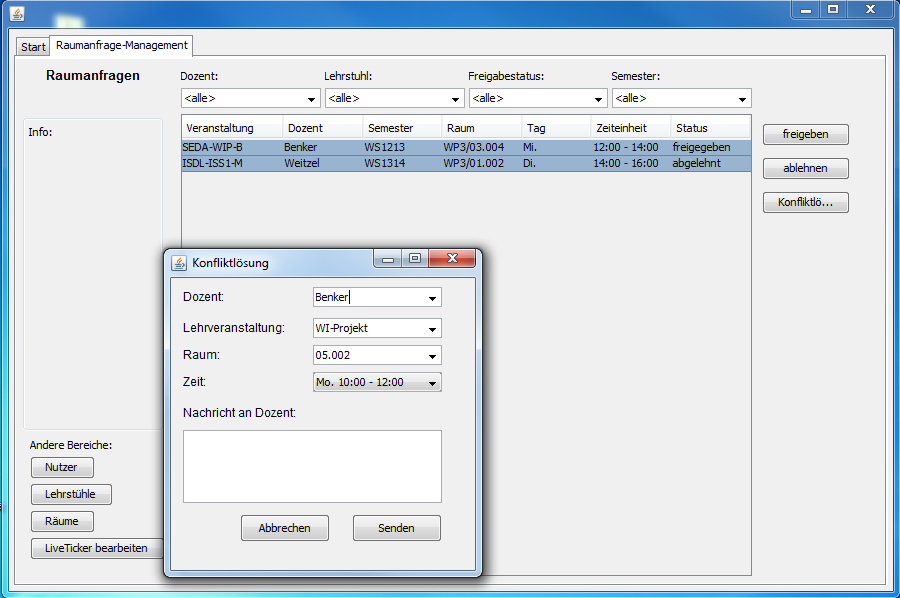
\includegraphics[width=150mm]{images/section_7/VerwaltungRaumanfragen.PNG}
\caption{Konfliktlösung der Raumanfragen}
\label{img:KonfliktlösungVerwaltung}
\end{center}
\end{figure}

\begin{figure}[H]
\begin{center}
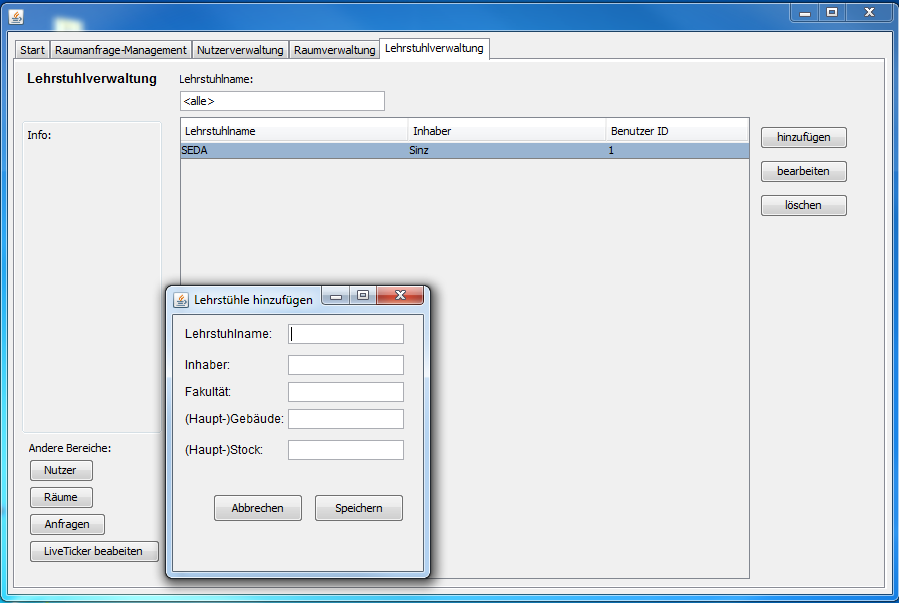
\includegraphics[width=150mm]{images/section_7/VerwaltungLehrstuhlverwaltung.PNG}
\caption{Verwaltung der Lehrstühle}
\label{img:LehrstuhlVerw}
\end{center}
\end{figure}

\begin{figure}[H]
\begin{center}
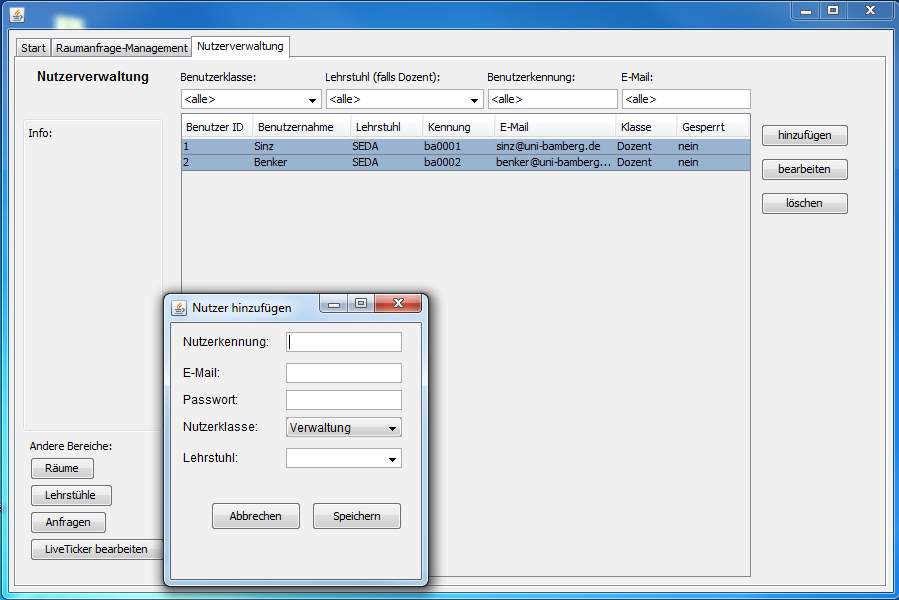
\includegraphics[width=150mm]{images/section_7/VerwaltungNutzerverwaltung.PNG}
\caption{Verwaltung der Nutzer}
\label{img:NutzerVerw}
\end{center}
\end{figure}

\begin{figure}[H]
\begin{center}
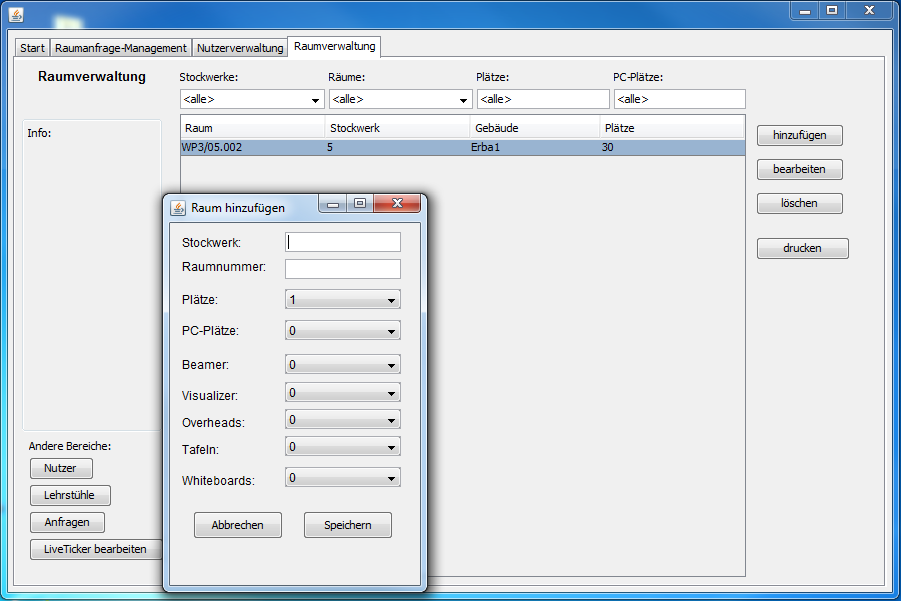
\includegraphics[width=150mm]{images/section_7/VerwaltungRaumverwaltung.PNG}
\caption{Verwaltung der Räume}
\label{img:RaumVerw}
\end{center}
\end{figure}


Die personalisierte Startseite der Dozenten beinhaltet zwei Listen [siehe Abbildung \ref{img:StartDoz}]. In der oberen werden alle Veranstaltungen visualisiert und können nach Lehrstühlen, Dozenten und Semester gefiltert werden. Außerdem wird der Veröffentlichungsstatus sowie die erfolgreich Raumanfrage angezeigt[siehe /F70/]. Eine weitere Liste gibt zusätzliche Auskunft zum Status der Raumanfragen/Raumzuordnungen. Bei einer erfolgreich durchgeführten Raumanfrage kann der jeweilige Dozent seine Lehrveranstaltung anschließend veröffentlichen. Die mit der Raumanfrage bezogenen Nachrichten der Hausverwaltung werden im Live-Ticker (links) angezeigt.
Um Lehrveranstaltungen zunächst überhaupt hinzuzufügen wird der Button "`hinzufügen"' gewählt und in einem neuen Fenster können Lehrstuhl und Dozent ausgewählt werden und somit die Bezeichnung neuer Veranstaltungen gesetzt werden [siehe /F20/ und siehe Abbildung \ref{img:LehrveranstaltungsVerwDoz}]. 
Um der Lehrveranstaltung einen Raum zuzuordnen, kann eine Raumanfrage über den Button "`Raumanfrage"' [siehe Abbild \ref{img:RaumanfrageDoz}] spezifiziert und versandet werden [siehe /F30/]. Hierfür kann entweder ein gewünschter Raum oder nur die besonderen Anforderungen an die Hausverwaltung zur weiteren Bearbeitung übermittelt werden.
Außerdem können die Aktionen eigener Stundenplan [siehe /F150/ und siehe Abbildung \ref{img:StundenplanDoz}] und Lehrstuhlplan [siehe /F140/ und siehe Abbildung \ref{img:LehrstuhlplanDoz}] sowie eine LiveTicker Bearbeitung (um bspw. Studenten veranstaltungs- oder lehrstuhlsbezogene Nachrichten anzeigen lassen zu können) [siehe /FW21/] gewählt werden.


\begin{figure}[H]
\begin{center}
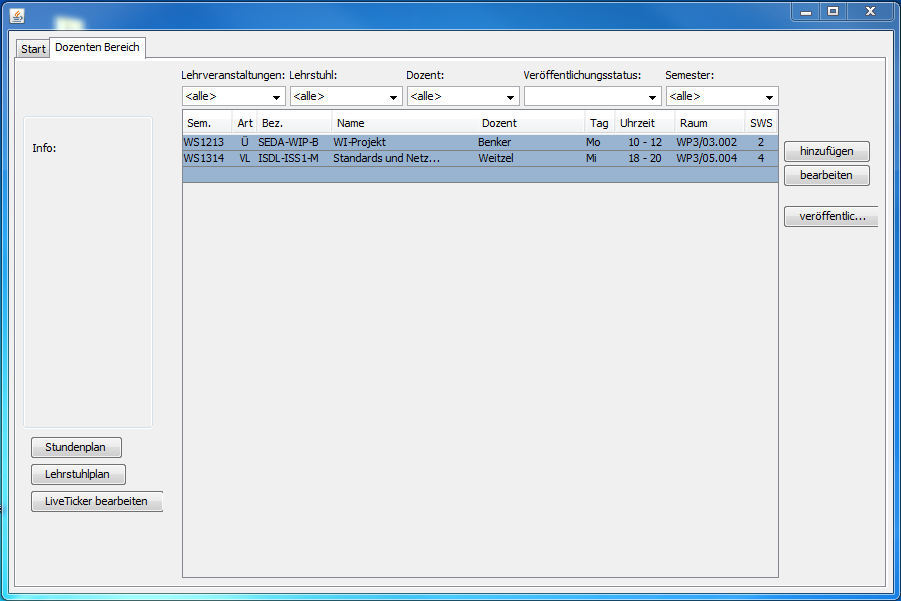
\includegraphics[width=150mm]{images/section_7/DozentenHauptseite.PNG}
\caption{Startseite für Dozenten}
\label{img:StartDoz}
\end{center}
\end{figure}



\begin{figure}[H]
\begin{center}
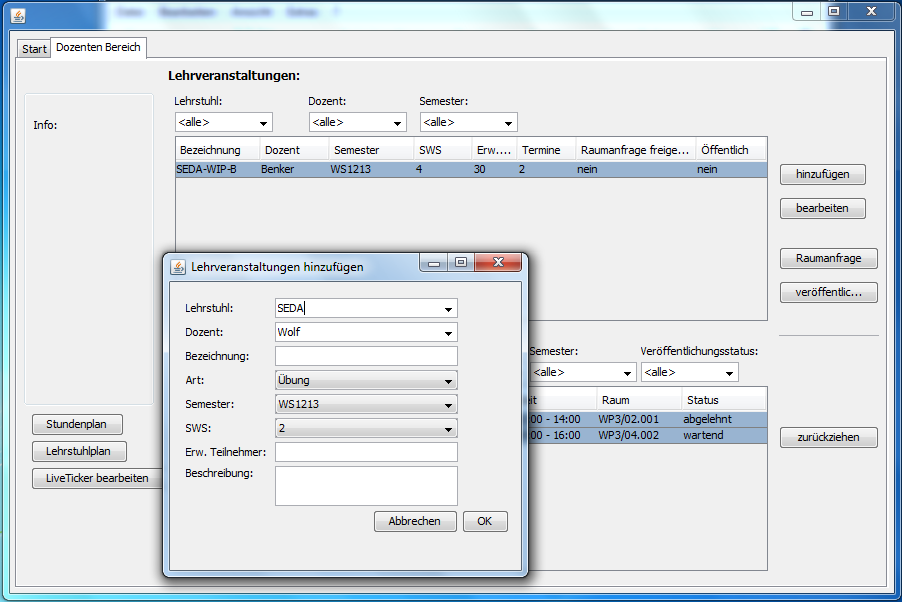
\includegraphics[width=150mm]{images/section_7/DozentenLehrveranstaltungenHinzufuegen.PNG}
\caption{Verwaltung der Lehrveranstaltungen durch die Dozenten}
\label{img:LehrveranstaltungsVerwDoz}
\end{center}
\end{figure}



\begin{figure}[H]
\begin{center}
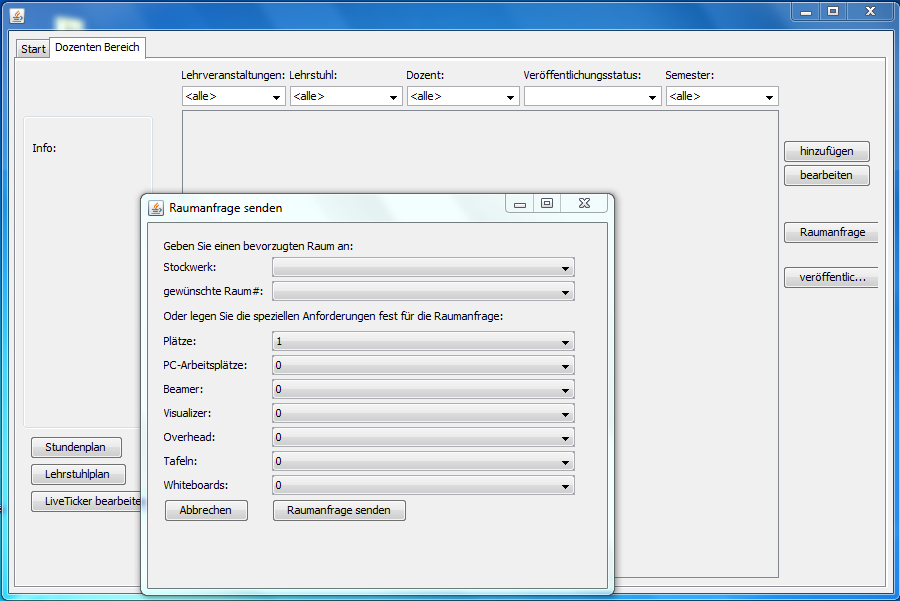
\includegraphics[width=150mm]{images/section_7/DozentenRaumanfrage.PNG}
\caption{Raumanfragen durch die Dozenten}
\label{img:RaumanfrageDoz}
\end{center}
\end{figure}


\newpage
\section{Preamble}
\label{sec:preamp}

We'd like to address the reader of this documentation before going into the details of this documentation that the project itself encountered several challenges which couldn't all be solved in a satisfying way. These lead to a program with a limited functionality and a documentation with some major gaps. For reasons and the progress itself which lead to this situation please refer to chapter 8.
\newpage
\section{Testszenarien}
\label{sec:Testszenarien}


Damit festgestellt werden kann, ob die Software auch einwandfrei funktioniert, müssen verschiedene Testszenarien durchlaufen werden.
Die Tests werden auf verschiedenen Ebenen ausgeführt. Unterschieden wird hierbei zwischen dem Modultest, Integrationstest, Systemtest und letztendlich dem Abnahmetest.
Im Folgenden werden nun diese Testszenarien genauer beschrieben und dargelegt, wie sie am 
Programm durchgeführt werden.
//
\begin{tabular}{p{1.5cm}p{14.5cm}}
 /T10/	& Im Komponententest, welcher wie auch der nachfolgende Modultest unter White-Box-Tests fällt, beinhaltet das Testen von einzeln abgrenzbaren Teilen (Modulen) des Gesamtprogramms. Das Testen erfolgt bei White-Box-Tests in der Entwicklungsumgebung Eclipse, wo der Quelltext sichtbar ist. Einzelne Klassen, Funktionen und Unterprogramme werden im Modultest dem Tester sequenziell unterworfen und auf Fehlerfreiheit geprüft. Dies umfasst unter anderem eine korrekte Ausgabe von Uhrzeiten. Auch SQL-Abfragen an die Datenbank ob die Passwortabfrage korrekt abgespeichert wurden, soll der Test beinhalten. \\[0.25cm]	 
\end{tabular}

\newpage
\section{Preamble}
\label{sec:preamp}

We'd like to address the reader of this documentation before going into the details of this documentation that the project itself encountered several challenges which couldn't all be solved in a satisfying way. These lead to a program with a limited functionality and a documentation with some major gaps. For reasons and the progress itself which lead to this situation please refer to chapter 8.
\newpage
\section{Preamble}
\label{sec:preamp}

We'd like to address the reader of this documentation before going into the details of this documentation that the project itself encountered several challenges which couldn't all be solved in a satisfying way. These lead to a program with a limited functionality and a documentation with some major gaps. For reasons and the progress itself which lead to this situation please refer to chapter 8.
\newpage
\section{Glossar}

%\newpage{Abkrzugsverzeichnis}
%\addcontentsline{toc}{chapter}{Abkrzungsverzeichnis}
%%\addcontentsline{toc}{chapter}{\protect{Glossar}}
\begin{acronym}[abkuerzungen2]
\acro{API}{Die API stellt eine dokumentierte Software-Schnittstelle dar, die von anderen Programmen aus genutzt werden kann.}
\acro{CLI}{Command Line Interface - Kommandozeile. Die Kommandozeile ist ein Eingabebereich für die Steuerung einer Software, die typischerweise im Textmodus abläuft.}
\acro{DNS}{Ermöglicht es Klarnamen in numerische IP Adressen (z.B. google-public-dns-a.google.com in 8.8.8.8 umzuwandeln).}
\acro{GUI}{Hierbei handelt es sich um die grafische Benutzeroberfläche.}
\acro{IP}{Ein Protokoll das für die Vermittlung von Daten dient.}
\acro{ISO}{Eine internationale Vereinigung von Normungsorganisationen.}
\acro{JDBC}{Hierbei handelt es sich um eine Datenbankschnittstelle für Java.}
\acro{Klasse}{Im Kontext der Programmierung handelt es sich hierbei um einen abgegrenzten Bereich (ein sogenanntes "`Objekt"') mit bestimmten Attributen und Methoden.}
\acro{LDAP}{Ein Verzeichnisdienst um Abfragen und Modifikationen von Informationen zu erlauben.}
\acro{ODBC}{Hierbei handelt es sich um eine Datenbankschnittstelle von Microsoft.}
\acro{RFC}{RFCs sind eine Reihe von technischen und organisatorischen Dokumenten zum Internet, die sie zu einem Standard entwickelt haben.}
\acro{Salt}{Ein Salt (zu Deutsch "`Salz"') wird bei der Erstellung einer Prüfsumme zu einem Passwort beigegeben, um zu gleichen Passwörtern unterschiedliche Prüfsummen zu erhalten. Ohne ein Salt wäre anhand der Prüfsumme das Passwort zu erkennen, wenn einmal bekannt ist, welche Prüfsumme zu welchem Passwort gehört.}
\acro{SHA-256}{SHA steht für "`Secure Hash Algorithm"' wobei die angefügte Zahl die Länge der generierten Prüfsumme ("`Hash"') in Bit angibt.}
\acro{Shell}{Eingabe-Schnittstelle zwischen Computer und Benutzer - meist grafisch}
\acro{SQL}{Eine deskriptive Abfragesprache von Datenbanken.}
\acro{TCP}{Ein verbindungsorientiertes Protokoll, um Daten im Netzwerk zu transportieren.}
\acro{UDP}{Ein verbindungsloses Protokoll, um Daten im Netzwerk zu transportieren.}
\end{acronym}

\newpage
\bibliography{references}
\end{document}
